% Section: parallel (\input from main.tex)
\section{A* in the Parallel World}
\label{sec:par}

\subsection{Why the two parts do not merge directly}

Using the sorted list of Section~\ref{sec:clist} as the OPEN list of the A* of
Section~\ref{sec:seq} fails for four reasons:

\begin{enumerate}[nosep]
  \item The list is a \emph{set} of distinct keys, but OPEN holds $(f, v)$
        pairs and many nodes share the same $f$.
  \item The list has no operation that removes the minimum.
  \item The CLOSED set and the $g$ and parent arrays would be read and written
        by several threads without synchronization.
  \item The two stopping rules of sequential A* become wrong. The first goal
        popped is not necessarily optimal, because another thread may still be
        expanding a cheaper node. An empty OPEN does not mean the search is
        over, because another thread may be about to insert children.
\end{enumerate}

\subsection{Adaptations}\label{sec:par-adapt}

\paragraph{The list.} The key becomes the 64-bit integer $(f \ll 24) \mid v$.
Keys are unique per node and $f$ value, and their order is the order of $f$.
Inserting the same node twice with the same $f$ is a harmless duplicate that
\texttt{add} rejects. \texttt{removeMin} was added to every list
(Section~\ref{sec:clist}).

\paragraph{The search.} There is no CLOSED set. The $g$-value and the parent of
each node are packed into one 64-bit \texttt{std::atomic} and lowered with a
compare-and-swap loop, so $g$ and parent always belong together. Whenever
$g(v)$ improves, $v$ is inserted again. A node can therefore be expanded more
than once; these extra expansions are the \emph{search overhead} of parallel
A*. A popped entry with $f > g(u) + h(u)$ is stale and skipped. An
\emph{incumbent} $U$ holds the cost of the best path to the goal found so far
(an atomic minimum). Entries with $f \ge U$ are neither inserted nor expanded.

\paragraph{Termination.} A counter \texttt{pending} holds the number of
outstanding work items: the entries in OPEN plus the entries that a thread has
popped and is still processing. It starts at 1 (the source). Before a thread
inserts the children of a node it reserves one item per outgoing edge; when all
children are in OPEN it releases the reservations it did not use together with
the popped entry itself. \texttt{pending} therefore never under-counts, and it
can reach zero only when OPEN is empty and no thread holds an entry, after
which no thread can create work any more. A thread that finds OPEN empty stops
the search exactly when \texttt{pending} is zero. Two separate reads (``OPEN is
empty'', then ``no thread is busy'') would not be enough: between the two reads
another thread can insert its children and finish, and the search would stop
with work left in OPEN. \texttt{push} reports whether the entry was really
added, because the list is a set and rejects a duplicate key.

\begin{lstlisting}
std::atomic<long> pending{1};                            // the source
while (!done.load(std::memory_order_acquire)) {
  Key k;
  if (!open.pop(k)) {                                    // removeMin
    if (pending.load() == 0) { done = true; break; }
    backoff(); continue;
  }
  Cost f = key_f(k); int u = key_v(k);
  Cost gu = unpack_g(G[u].load(std::memory_order_acquire));
  if (f > gu + h(u) || f >= U.load()) { pending.fetch_sub(1); continue; } // stale / pruned
  if (u == t) { atomic_min(U, gu); pending.fetch_sub(1); continue; }
  long reserved = graph.degree(u), added = 0;
  pending.fetch_add(reserved);                           // before any child is inserted
  for (auto e = graph.begin(u); e != graph.end(u); ++e) {
    Cost ng = gu + e->w;
    if (cas_min_g(G[e->to], ng, u)) {                    // g and parent in one CAS
      if (e->to == t) atomic_min(U, ng);
      if (ng + h(e->to) < U.load() && open.push(make_key(ng + h(e->to), e->to))) added++;
    }
  }
  pending.fetch_sub(reserved - added + 1);               // unused reservations + this entry
}
\end{lstlisting}

\paragraph{Why the result is optimal.} When the search stops, \texttt{pending} is
zero: OPEN is empty and no thread is expanding, so every node whose $g$ was ever lowered to a value
with $f < U$ has been expanded with its final $g$. Take an optimal path
$s = v_0, \dots, v_k = t$ and suppose some node on it ends with
$g(v_i) > g^*(v_i)$; take the first one. Its predecessor ended with the optimal
$g^*(v_{i-1})$ and, because $h$ is consistent, with
$f \le C^* \le U$, so it was expanded and lowered $g(v_i)$ to $g^*(v_i)$ ---
a contradiction. Hence $g(t) = C^*$. The parent chain is a real path of that
cost: if a parent's final $g$ plus the edge cost were smaller than its child's
$g$, the parent would have been expanded again and would have improved the
child.

\subsection{Versions compared}

\begin{center}
\small
\begin{tabularx}{\linewidth}{>{\raggedright\arraybackslash}p{3.6cm} >{\raggedright\arraybackslash}p{3.3cm} Y}
\toprule
\textbf{Version} & \textbf{OPEN list} & \textbf{Notes} \\
\midrule
sequential A*   & binary heap & Section~\ref{sec:seq}; baseline for all speed-ups \\
list: coarse / fine / optimistic / lazy & shared sorted list & the adapted lists of Part~2, each with \texttt{std::mutex} and with TTAS+backoff (8 versions) \\
shared heap     & binary heap + one lock & $O(\log n)$ operations, but one lock serializes everything \\
\HDA            & one private heap per thread & Hash-Distributed A*~[5]: node $v$ belongs to thread $\mathrm{hash}(v) \bmod T$; generated nodes are sent in batches to the owner's mailbox; termination through a global count of outstanding work \\
\HDA{} + $f$-window & as \HDA & a thread waits while its best $f$ is more than 3\% above the smallest $f$ published by any thread (Section~\ref{sec:opt}) \\
\bottomrule
\end{tabularx}
\end{center}

\subsection{Correctness testing}

\texttt{test\_par} picks 30 random $(s, t)$ pairs on the city graph (one with
$s = t$) and runs 11 version/heuristic combinations with 1, 2, 4 and 8
threads: 1\,320 runs per platform and 3\,960 in total. Every run must return
\emph{exactly} the Dijkstra-optimal cost, and its path must start at $s$, end
at $t$, use only existing edges and have an edge sum equal to the returned
cost. The different thread counts and repeated runs exercise many
interleavings, and 8 threads on 2 or 4 cores force threads to be preempted
inside critical sections. The suite was also run under ThreadSanitizer.

All 3\,960 runs pass and ThreadSanitizer reports no data race. In the
benchmarks below, the mean and the worst cost/optimum ratio are 1.000000 for
every version, so the versions differ only in time.

\subsection{Results}

Each benchmark answers 20 long queries (straight-line distance $> 5$\,km;
about 100\,000 Dijkstra expansions each). We measured four heuristics:
$h = 0$ (parallel Dijkstra), Euclidean, ALT with 8 landmarks, and a
\emph{costly} heuristic. The costly heuristic returns the Euclidean value but
performs 400 dependent floating-point operations per evaluation (about
0.5--1\,$\mu$s). It stands for an expensive predictor, such as a learned
travel-time model, and lets us vary the amount of work per expansion. With
$h = 0$ the list versions were left out: with OPEN lists of thousands of
entries they would take hours.

\begin{figure}[H]
\centering
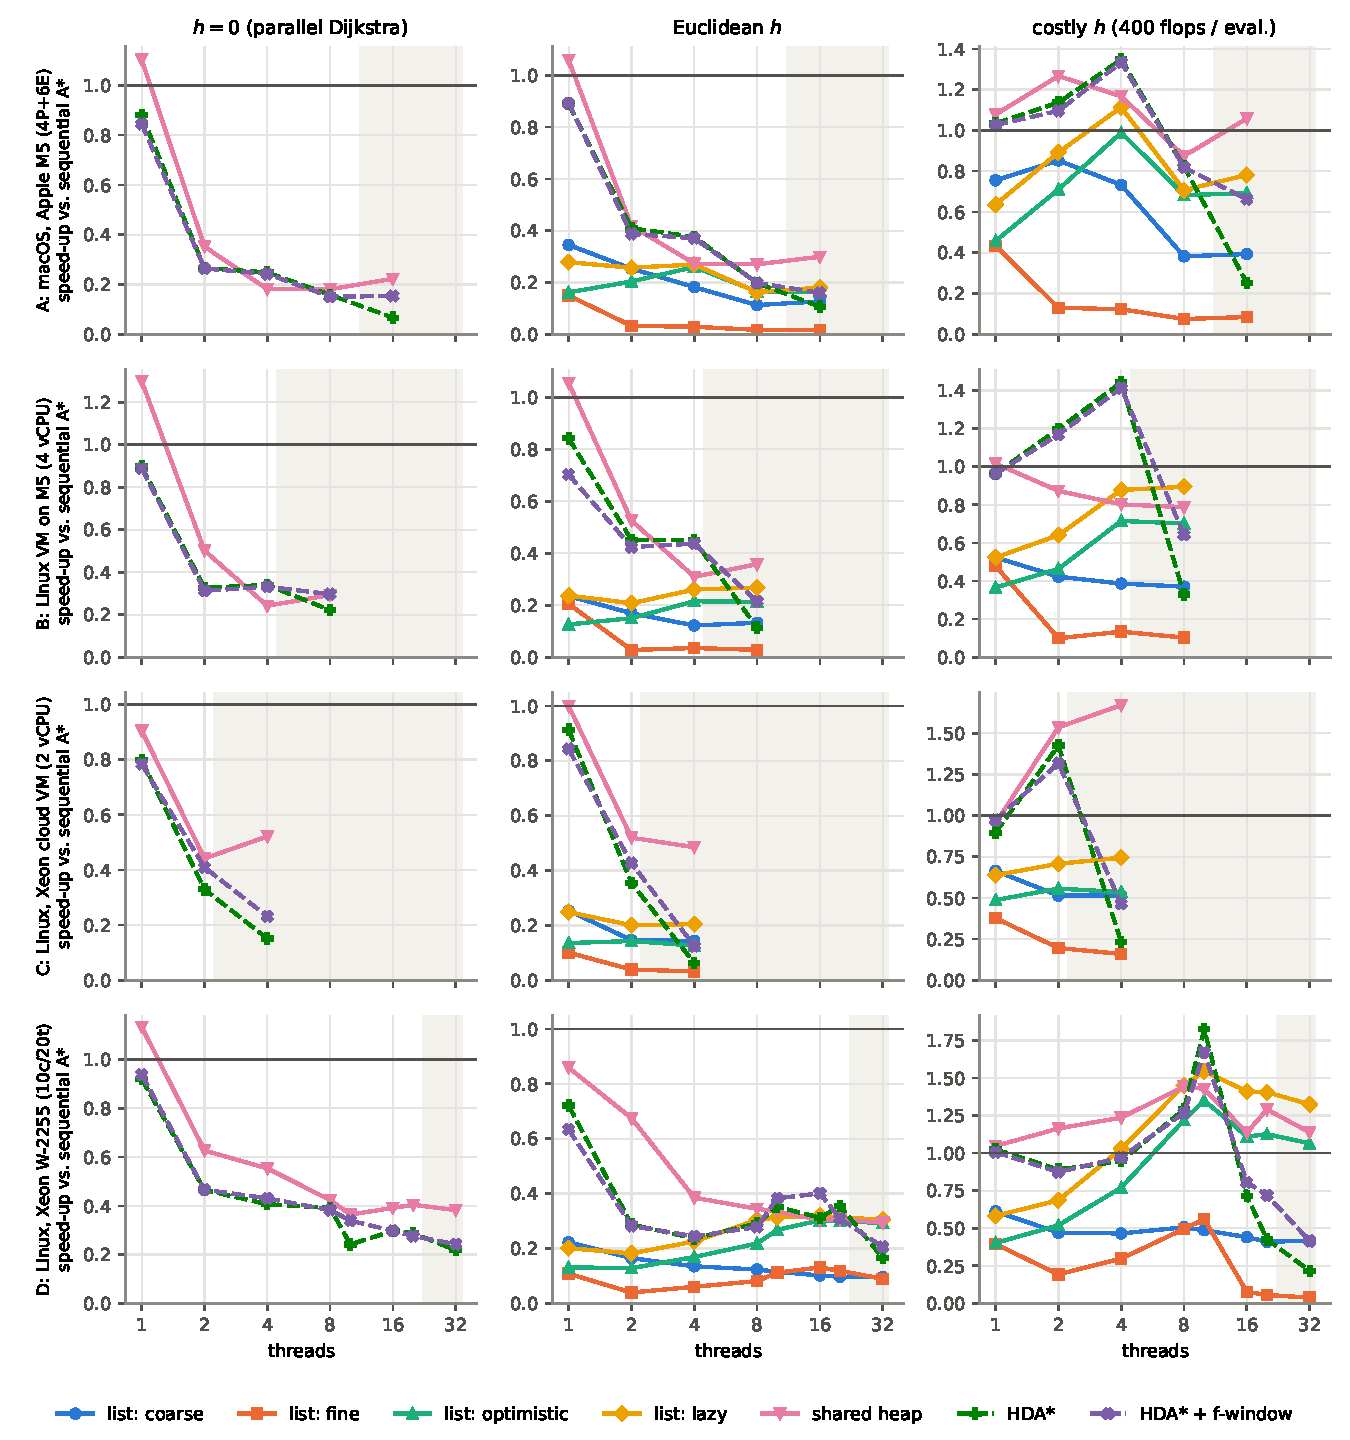
\includegraphics[width=\linewidth]{figures/fig6_astar.pdf}
\caption{Part 3: speed-up of parallel A* over sequential A* on the three
platforms (rows) for three heuristics (columns); 20 long queries, median of 3
runs. Solid lines: shared OPEN list (lists and heap with TTAS+backoff); dashed:
\HDA. The shaded region marks oversubscription.}
\label{fig:astar}
\end{figure}

\begin{table}[H]
\centering
\scriptsize
\setlength{\tabcolsep}{4pt}
\caption{Part 3: wall time (ms) to answer 20 long queries. Bold: faster than
sequential A* on the same platform. Locks are TTAS+backoff unless stated.}
\label{tab:astar}
\begin{tabular}{lrrrrrrrrrr}
\toprule
 & \multicolumn{5}{c}{Euclidean $h$ (threads)} & \multicolumn{5}{c}{costly $h$ (threads)} \\
\cmidrule(lr){2-6}\cmidrule(lr){7-11}
Version & 1 & 2 & 4 & 8 & 16 & 1 & 2 & 4 & 8 & 16 \\
\midrule
\multicolumn{11}{l}{\emph{Platform A (macOS, Apple M5)}} \\
sequential A* & 40 &  &  &  &  & 169 &  &  &  &  \\
list: coarse & 115 & 157 & 218 & 353 & 312 & 224 & 198 & 231 & 442 & 429 \\
list: fine & 265 & 1229 & 1379 & 2374 & 2674 & 390 & 1303 & 1376 & 2267 & 2002 \\
list: optimistic & 246 & 195 & 153 & 241 & 241 & 369 & 238 & 171 & 247 & 244 \\
list: lazy & 143 & 154 & 147 & 243 & 221 & 266 & 189 & \textbf{152} & 239 & 216 \\
list: lazy, \texttt{std::mutex} & 156 & 276 & 273 & 442 & 428 & 279 & 298 & 285 & 475 & 451 \\
shared heap & \textbf{37} & 95 & 145 & 147 & 132 & \textbf{157} & \textbf{133} & \textbf{145} & 193 & \textbf{160} \\
shared heap, \texttt{std::mutex} & \textbf{40} & 96 & 151 & 228 & 210 & \textbf{158} & 246 & 251 & 409 & 346 \\
HDA* & 45 & 97 & 105 & 200 & 373 & \textbf{163} & \textbf{149} & \textbf{125} & 205 & 670 \\
HDA* + $f$-window & 44 & 102 & 107 & 200 & 248 & \textbf{164} & \textbf{154} & \textbf{127} & 206 & 255 \\
\midrule
\multicolumn{11}{l}{\emph{Platform B (Linux VM, 4 vCPU)}} \\
sequential A* & 39 &  &  &  &  & 143 &  &  &  &  \\
list: coarse & 166 & 231 & 319 & 294 & -- & 273 & 338 & 370 & 386 & -- \\
list: fine & 190 & 1394 & 1101 & 1370 & -- & 298 & 1433 & 1065 & 1385 & -- \\
list: optimistic & 309 & 259 & 181 & 183 & -- & 390 & 308 & 200 & 203 & -- \\
list: lazy & 164 & 188 & 150 & 145 & -- & 273 & 223 & 163 & 160 & -- \\
list: lazy, \texttt{std::mutex} & 194 & 191 & 179 & 179 & -- & 287 & 235 & 195 & 191 & -- \\
shared heap & \textbf{37} & 74 & 126 & 109 & -- & \textbf{141} & 164 & 178 & 181 & -- \\
shared heap, \texttt{std::mutex} & \textbf{38} & 127 & 137 & 154 & -- & \textbf{143} & 270 & 252 & 258 & -- \\
HDA* & 46 & 86 & 87 & 343 & -- & 148 & \textbf{119} & \textbf{99} & 434 & -- \\
HDA* + $f$-window & 55 & 92 & 89 & 181 & -- & 148 & \textbf{122} & \textbf{101} & 222 & -- \\
\midrule
\multicolumn{11}{l}{\emph{Platform C (Linux, Xeon, 2 vCPU)}} \\
sequential A* & 91 &  &  &  &  & 464 &  &  &  &  \\
list: coarse & 360 & 624 & 636 & -- & -- & 699 & 902 & 900 & -- & -- \\
list: fine & 907 & 2329 & 2831 & -- & -- & 1232 & 2368 & 2904 & -- & -- \\
list: optimistic & 673 & 638 & 723 & -- & -- & 953 & 834 & 867 & -- & -- \\
list: lazy & 367 & 456 & 446 & -- & -- & 727 & 656 & 624 & -- & -- \\
list: lazy, \texttt{std::mutex} & 455 & 490 & 581 & -- & -- & 848 & 686 & 703 & -- & -- \\
shared heap & 91 & 176 & 188 & -- & -- & 486 & \textbf{302} & \textbf{278} & -- & -- \\
shared heap, \texttt{std::mutex} & \textbf{91} & 455 & 157 & -- & -- & 501 & 549 & \textbf{400} & -- & -- \\
HDA* & 100 & 257 & 1449 & -- & -- & 518 & \textbf{326} & 1996 & -- & -- \\
HDA* + $f$-window & 108 & 214 & 730 & -- & -- & 477 & \textbf{352} & 999 & -- & -- \\
\bottomrule
\end{tabular}

\end{table}

\textbf{With a cheap heuristic, no parallel version is faster.} With the
Euclidean or ALT heuristic, or with $h = 0$, one expansion takes about
0.2--0.4\,$\mu$s: three or four edges and a few array accesses. That is about
the cost of one operation on the shared OPEN list, plus the cache misses on
its head. Adding threads therefore adds synchronization and cache-coherence
traffic faster than it adds useful work. From 2 threads on, every version
runs at 0.79$\times$ the speed of sequential A* or slower, on every platform
(Figure~\ref{fig:astar}, left and middle columns).

\textbf{A sorted list is a poor priority queue on a large graph.} Even with
one thread the list versions are 3--14$\times$ slower than the binary heap
with the Euclidean heuristic. Insertion walks the list, so it costs
$O(|\textrm{OPEN}|)$ instead of $O(\log |\textrm{OPEN}|)$, and on the city
graph OPEN holds thousands of nodes. The gap shrinks as the heuristic gets
better (ALT: 1.4--4$\times$), because a better heuristic keeps OPEN smaller.
With more threads every \texttt{removeMin} also competes for the head of the
list, which is exactly the priority-queue bottleneck measured in Part~2. The
ranking of the lists is the same as in Part~2: lazy (and optimistic) with
backoff are the best, fine-grained is by far the worst.

\textbf{Parallelism pays off only when expansions are expensive.} With the
costly heuristic (right column), several versions beat sequential A*: \HDA{}
reaches $1.35\times$ on Platform~A and $1.44\times$ on B (both at 4 threads),
and the shared heap with backoff reaches $1.27\times$ on A and $1.67\times$ on
C. On a large graph the lists also profit from more threads, because several
threads can walk the long list at the same time: on Platform~A the lazy list
goes from $0.64\times$ with one thread to $1.11\times$ with 4, the first
list-based parallel A* that is faster than sequential A*, and the optimistic
list from $0.46\times$ to $0.99\times$. On Platform~A every version slows down
again beyond 4 threads, although the machine has 10 cores: only 4 of them are
performance cores, and in a search that all threads share, the slowest thread
holds the others back. \texttt{std::mutex} is never the better lock here (lazy
list on A: $0.59\times$ against $1.11\times$ with backoff at 4 threads),
because the critical sections last only a few hundred nanoseconds, much less
than a sleep and wake-up in the kernel.

\begin{figure}[H]
\centering
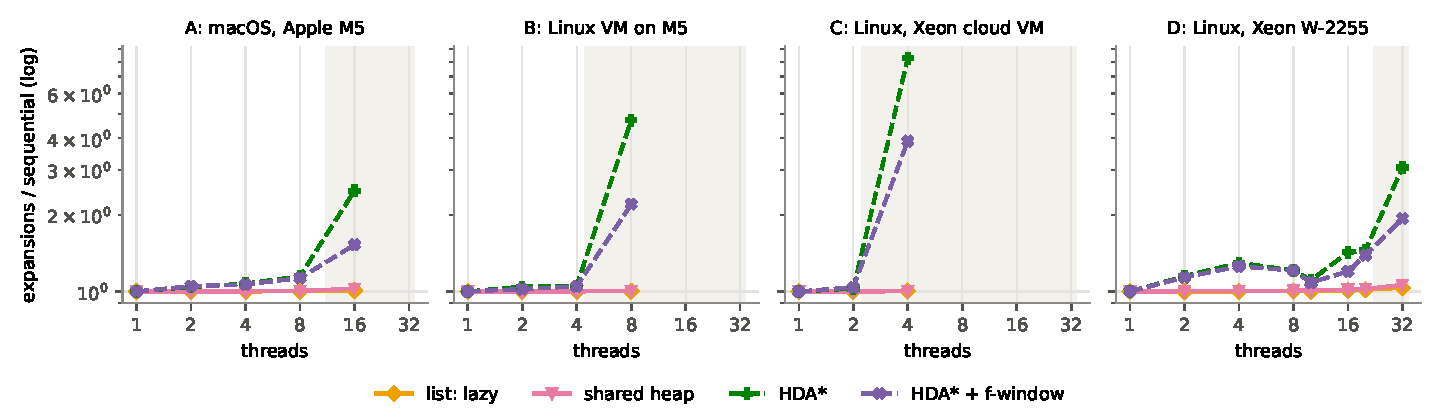
\includegraphics[width=\linewidth]{figures/fig7_overhead.pdf}
\caption{Part 3: search overhead with the Euclidean heuristic: expanded nodes
divided by those of sequential A*. Shaded: oversubscription.}
\label{fig:overhead}
\end{figure}

\textbf{\HDA{} trades contention for search overhead.} \HDA{} has no shared
OPEN list, so it does not suffer the bottleneck at the head. It also has no
global $f$-order, and Figure~\ref{fig:overhead} shows the price. While every
thread has its own core it expands at most 15\% more nodes than sequential A*
with the Euclidean heuristic. When a thread is descheduled, the nodes it owns
stop moving, the path to the goal stalls, and the other threads keep expanding
nodes far beyond the optimal $f$ because $U$ is still infinite: on Platform~C
\HDA{} expands $8\times$ more nodes than sequential A* at 4 threads ($21\times$
with ALT). The shared OPEN list stays within 20\% at every thread count,
because its threads always take the globally best node.
